\newpage\vspace*{-21.6pt}
\section{绪论}%每一个一级标题(\section)单独起页;
\subsection{写给读者}
本\LaTeX 模板格式完全参考原Word模板“附件7:中南大学毕业设计(论文)模板.docx”,是由作者(本科学生)自己编写的\LaTeX 模板,不是官方书写的模板。

本\LaTeX 模板适用于对\LaTeX 具有一定程度了解的读者,对新手可能不友好:对\LaTeX 各类环境命令不熟悉,或在编译过程中出现的问题不能及时解决,其排版效率将远不如Word。作者认为,读者至少已经看完了流行的入门教程《112分钟学会\LaTeX 》。

\subsection{\LaTeX 与Word的比较}
先写在前面,就作者长期作用\LaTeX 和Word 进行科技论文或一般文章的书写排版的经验来看:作为文字书写和排版工具,综合来看,\textcolor{red}{Word 或WPS 是要强于\LaTeX 的}。

\subsubsection{\LaTeX 的特点}
\LaTeX 是一种基于\TeX 的文档排版系统,为减轻写作、排版一肩挑的负担,将大片排版的格式细节隐藏在若干样式之后,是现在最流行的科技写作——尤其是数学写作的工具之一。

相比Word,在公式编辑的格式控制、公式编辑的易用程度与编辑效率(包括作者,在Word中编辑公式时,仍然使用MathType中的\TeX 输入方式)、交叉引用、文献管理上,\LaTeX 要比Word 好用太多,可以说是全面胜出,所以学术圈更青睐于\LaTeX 。

漂亮。不少文字排版工作者都认为用\LaTeX 书写出来的文章要比Word好看很多。

在有现成模板的情况下,\LaTeX 模板用起来比Word模板更方便。

\LaTeX 系统是免费的,而Word和MathType是商业软件,对于大部分人而言(至少本科生),收费高昂。

\subsubsection{Word的特点}
但Word的优点在诸多方面远远胜于\LaTeX :

简单,易上手。Word除了书写正文需要敲敲键盘,排版可能只需要点一点鼠标。由于“所见即所得”,Word上手难度极小,简单易懂。而\LaTeX 具有大量让人望而生畏的代码,有烦人的debug,如果只学习了部分\LaTeX 环境命令的知识,可能难以排版出一篇合格的文章。

Word本身有文字编辑上的辅助功能,而一般\LaTeX 编辑器只有代码书写辅助功能(还很鸡肋),对于大段纯文字的写作,完全没必要使用\LaTeX 。

Word在表格上编辑排版略胜于\LaTeX 。

\subsection{本章小节}
刘海洋老师在《\LaTeX 入门》一书中写到:“\LaTeX 是一种并不简单的计算机语言,不能只点点鼠标就弄好一篇漂亮的文章,也不是一两个小时的泛泛了解就尽能对付得过去。”

对于元素众多,格式复杂的文章,\LaTeX 可能更胜Word一筹,但对于大部分时间遇到的文章,Word远优于\LaTeX 。

本\LaTeX 模板可运用CTeX+WinEdt 或CTeX+TeXstudio进行编译和编辑。

\newpage\vspace*{-21.6pt}
\section{组织你的文本}
从本章开始,对论文中可能出现的各类\,\LaTeX 环境与命令进行说明,主要包括文字与符号、论文的结构层次、图表的绘制、自动化工具(目录格式与文献格式)进行说明。

\subsection{文字与说明}
正文中文使用小四宋体,英文使用Times New Roman字体。其余特殊环境字体大小在后文中说明。

行距为word中的1.5倍行距,总行距为$1.5\times 1.2\times 12\mathrm{pt} $。

\subsection{段落与文本环境}
\subsubsection{列表环境}
文中可以使用列表:
\begin{enumerate}
  \item 中文
  \item 英语
  \item 法语
\end{enumerate}

也可以使用下列更常用和紧凑的一个定制格式:
\begin{enumerate}[itemsep=0pt,parsep=0pt,label=(\arabic*)]
  \item 中文
  \item 英语
  \item 法语
\end{enumerate}

\subsubsection{脚注环境}
在正文中可以使用脚注进行文字说明,同时对原\LaTeX 中默认的脚注编号格式进行了优化,例如\footnote{这是一个更好的带圆圈的脚注}。

\subsubsection{程序代码环境}
当你的论文中有程序代码需要列出时,可以使用作者为你定制的程序代码环境,见附录。当然,这里只对Matlab语言进行了设置,对于其它常见语言(C++、Python等),读者可以自行进行关键字高亮、字体大小等进行设置。

\textcolor{red}{注意:在排版程序时,如果您的程序中包含中文字符,请使用规避符“}\verb"` `"\textcolor{red}{”:}

\verb"n=2000;%`投针次数figure;`"

\subsection{文档的结构层次}
与原Word版的文档结构层次相同,划分为章、节和小节三部分。读者只需分别在\verb"\section{}"、\verb"\subsection{}"和\verb"\subsubsection{}"中填入标题即可,如\\
\verb"\section{概论}"产生“第1章\quad 概论”,无需加“第1章”字样。

\textcolor{red}{注意,由于一级标题要求另起一页开始且分行,所以应在}\verb"\section{}"\textcolor{red}{命令前加}\verb"\newpage\vspace*{-21.6pt}"\textcolor{red}{命令。}

$21.6\mathrm{pt}$\,是小四字体($12\mathrm{pt}$)的1.5倍行距:$12\mathrm{pt}\times 1.2\times 1.5 = 21.6\mathrm{pt}$。

三层标题的字体大小及缩进与原Word模板无异。读者无需更改。

\subsection{页面格式设计}
\subsubsection{页边距}
左页边距为$3.0\mathrm{cm}$、右页边距为$2.0\mathrm{cm}$,且全文使用双面打印格式(\verb"twoside"),即单页左3右2,双页左2右3,修复了原Word模板中双面打印左右边距错误,不便装订的问题。

由于\LaTeX 与Word中计算上下页边距的方式不同(\LaTeX 上下边距包含了页眉页脚,而Word相反),故在\LaTeX 中将页眉页脚的距离计算了进来。

最终导言区geometry宏包中的页边距命令为:

\verb"a4paper,left=3.0cm,right=2.0cm,top=3.51cm,bottom=4.25cm"

\subsubsection{页眉和页脚}
页眉和页脚的格式与原Word模板相同。同时作者默认只有“摘要”、“ABSTRACT”和“目录”三部分使用罗马字体页码。

\newpage\vspace*{-21.6pt}
\section{自动化工具}
\subsection{目录格式}
目录格式在原Word模板格式的基础上额外添加了“摘要”、“ABSTRACT”和“目录”三部分,如不需要,则将“THSIS\_csu.tex”或“abstract.tex”文件中的

\verb"\phantomsection"

\verb"\addcontentsline{toc}{section}{摘要}"

等命令注释掉或删除。

本\LaTeX 模板与原Word模板中的目录各级标题的字体与缩进无异,但一级标题不是“第1章\quad 概论”,而是“1\quad 概论”,因为作者未能在titletoc宏包中找到类似设置,读者如有能力,请自行设置。

本模板中导言区titletoc宏包的设置命令如下:

\verb"\usepackage{titletoc}"

\verb"\titlecontents{section}[0mm]{}{}{}{}[]"

\verb"\dottedcontents{section}[0.0em]{\normalsize}{1.0em}{4pt}"

\verb"\dottedcontents{subsection}[3.0em]{\normalsize}{2.0em}{4pt}"

\verb"\dottedcontents{subsubsection}[6.0em]{\normalsize}{3.0em}{4pt}"

\subsection{交叉引用}
本模板生成的pdf文件中包含书签,方便电子档阅读,如使用SumatraPDF:“查看”$\to$“书签”。

目录、图表的标题、文献引用和URL地址都添加了彩色超链接功能,对于目录、图表的标题和文献引用为蓝色,而URL地址为洋红色。

其中,文献引用中:在正文中点击文献引用编号“[1]”,可链接至该条参考文献,在该条参考文献后有另一超链接,为该条文献引用的位置页码,例\cite{Meta_CN}。

如希望采用黑色超链接(特别是需要打印时),请在导言区hyperrdf宏包设置中更改\,\verb"colorlinks = true"为\,\verb"colorlink = false"。

同时在hyperrdf宏包设置中更改以下内容:

\verb"pdftitle = {中南大学本科毕业论文LaTeX模板},"

\verb"pdfauthor = {Chai Xingtao}"

上述两条为生成的PDF文档属性。

\subsection{文献格式}
文献格式采用国家标准GB/T 7714-2015格式,格式宏包和格式文件见\\
“gbt7714.sty”、“gbt7714-plain.bst”和“gbt7714-unsrt.bst”。

本模板使用\LaTeX 常用的\BibTeX 进行文献管理。

\newpage\vspace*{-21.6pt}
\section{图表的绘制}
\subsection{公式格式}
本\LaTeX 模板中的公式字体和大小、公式编号与原Word模板无异。例如:

对于三维、瞬态、可压缩牛顿流体的流动与传热现象,其守恒控制方程见如下:

质量守恒方程见式\,(\ref{equ:zhiLiang})。

\begin{equation}\label{equ:zhiLiang}
\frac{\partial\rho}{\partial t}+div\left(\rho u\right)=0
\end{equation}

$X$、$Y$和$Z$方向动量守恒方程分别见式\,(\ref{equ:dongLiangX})、式\,(\ref{equ:dongLiangY})和式\,(\ref{equ:dongLiangZ})。

\begin{equation}\label{equ:dongLiangX}
\frac{\partial\left(\rho u\right)}{\partial t} + div\left(\rho uu\right)=div\left(\mu\mathrm{grad}u\right)-\frac{\partial P}{\partial x}+S_u
\end{equation}

\begin{equation}\label{equ:dongLiangY}
\frac{\partial\left(\rho v\right)}{\partial t} + div\left(\rho vu\right)=div\left(\mu\mathrm{grad}v\right)-\frac{\partial P}{\partial y}+S_v
\end{equation}

\begin{equation}\label{equ:dongLiangZ}
\frac{\partial\left(\rho w\right)}{\partial t} + div\left(\rho wu\right)=div\left(\mu\mathrm{grad}w\right)-\frac{\partial P}{\partial z}+S_w
\end{equation}

能量守恒方程见式\,(\ref{equ:nengLiang})。
\begin{equation}\label{equ:nengLiang}
\frac{\partial\left(\rho T\right)}{\partial t}+div\left(\rho uT\right)=div\left(\frac{k}{c}\mathrm{grad}T\right)+S_T
\end{equation}

另,积分符号进行了优化,在原amsmath宏包中倾斜积分符号更改为了直立体:

\begin{equation}\label{equ:int}
  \int_0^{2\uppi}\sin x = 0
\end{equation}

\subsection{表格格式}

正文中所有表格均采用三线表,例如表\,(\ref{tab:test1})。为文章紧凑,所有表格均采用浮动体。

\textcolor{red}{注意:在浮动体中应更改字体大小,添加}\verb"\small"\textcolor{red}{命令,在}\verb"\caption{}"\textcolor{red}{中添加命令}\verb"\heiti "\textcolor{red}{命令。}

\begin{table}[htbp]
\small
  \centering
  \caption{\heiti 森林生态系统服务价值的敏感系数}\label{tab:test1}
    \begin{tabularx}{\textwidth}{cYYY}
    \toprule
    \phantom{year}Year\phantom{year}  & $CIF_f$  & $CIF_p$  & $CIF_g$ \\
    \midrule
    2006  & 7.4   & 2.59  & 0.07 \\
    2007  & 2.54  & 19.32 & 0.48 \\
    2008  & 6.07  & 12.78 & 11.56 \\
    2009  & 1.78  & 20.14 & 0.38 \\
    2010  & 1.32  & 0.61  & 0.12 \\
    2011  & 1.64  & 2.9   & 0.2 \\
    2012  & 1.02  & 12.57 & 1.38 \\
    \bottomrule
    \end{tabularx}
\end{table}

当表中行数较多,可以使用表格间隔底纹,见表\,(\ref{tab:test2})。
\begin{table}[htbp]
\small
  \centering
  \caption{\heiti 森林生态系统服务价值的敏感系数}\label{tab:test2}
    \begin{tabularx}{\textwidth}{cYYY}
    \toprule
    \phantom{year}Year\phantom{year}  & $CIF_f$  & $CIF_p$  & $CIF_g$ \\
    \midrule
    2006  & 7.4   & 2.59  & 0.07 \\
        \rowcolor{mygray}
    2007  & 2.54  & 19.32 & 0.48 \\
    2008  & 6.07  & 12.78 & 11.56 \\
        \rowcolor{mygray}
    2009  & 1.78  & 20.14 & 0.38 \\
    2010  & 1.32  & 0.61  & 0.12 \\
        \rowcolor{mygray}
    2011  & 1.64  & 2.9   & 0.2 \\
    2012  & 1.02  & 12.57 & 1.38 \\
    \bottomrule
    \end{tabularx}
\end{table}

另书写论文中常用的几个表格格式,见表\,(\ref{tab:ZhuChengFenJieGuo})、表\,(\ref{tab:PaiMIng})和表\,(\ref{tab:yi})

\begin{table}[htbp]
\footnotesize
  \centering
  \caption{\heiti 主成分分析结果}\label{tab:ZhuChengFenJieGuo}
  \begin{tabularx}{\textwidth}{cYYY||cYYY}
    \toprule
    % after \\: \hline or \cline{col1-col2} \cline{col3-col4} ...
    序号 & 特征根 & 贡献率 & \multicolumn{1}{c||}{累积贡献率} & 序号 & 特征根 & 贡献率 & 累积贡献率 \\
    \hhline{----||----}
    1 & 6.2865 & 48.3575  & 48.3575 & 8 & 0.1067 & 0.8210 &  98.8545 \\
    2 & 2.7959 & 21.5067 & 69.8642 & 9 & 0.0663 & 0.5102 &  99.3647 \\
    3 & 2.0499 & 15.7685 & 85.6327 & 10 & 0.0509 & 0.3914 & 99.7561 \\
    4 & 0.7560 & 5.8152 & 91.4479 & 11 & 0.0136 & 0.1044 & 99.8605 \\
    5 & 0.3919 & 3.0146 & 94.4625 & 12 & 0.0106 & 0.0813 & 99.9418 \\
    6 & 0.2543 & 1.9564 & 96.4188 & 13 & 0.0076 & 0.0582 & 100.0000 \\
    7 & 0.2099 & 1.6146 & 98.0335 &   &   &   &   \\
    \bottomrule
  \end{tabularx}
\end{table}

\begin{table}[htbp]
\footnotesize
  \centering
  \caption{\heiti 排名和综合结果}\label{tab:PaiMIng}
  \begin{tabular}{ccccccccc}
    \toprule
    % after \\: \hline or \cline{col1-col2} \cline{col3-col4} ...
    地区 & 广东 & 江苏 & 山西 & 浙江 & 河南 & 湖南 & 上海 & 湖北 \\
    \midrule
    名次 & 1 & 2 & 3 & 4 & 5 & 6 & 7 & 8 \\
    综合评价值 & \phantom{-}3.1511  &  \phantom{-}3.0754 &   \phantom{-}2.1268 &   \phantom{-}1.7027  &  \phantom{-}0.7627 &   \phantom{-}0.6234 &   \phantom{-}0.4570  &  \phantom{-}0.4079 \\
    \bottomrule
  \end{tabular}
  \begin{tabular}{ccccccccc}
    \toprule
    % after \\: \hline or \cline{col1-col2} \cline{col3-col4} ...
    地区 & 河北 & 北京 & 四川 & 安徽 & 辽宁 & 福建 & 天津 & 江西 \\
    \midrule
    名次 & 9 & 10 & 11 & 12 & 13 & 14 & 15 & 16 \\
    综合评价值 & \phantom{-}0.3821  &  \phantom{-}0.3371 &   \phantom{-}0.3144  &  \phantom{-}0.2034 &   \phantom{-}0.1928  &  \phantom{-}0.1223  &  \phantom{-}0.1004  &  -0.2223  \\
    \bottomrule
  \end{tabular}
  \begin{tabular}{ccccccccc}
    \toprule
    % after \\: \hline or \cline{col1-col2} \cline{col3-col4} ...
    地区 & 重庆 & 陕西 & 吉林 & 黑龙江 & 广西 & 山西 & 内蒙古 & 云南 \\
    \midrule
    名次 & 17 & 18 & 19 & 20 & 21 & 22 & 23 & 24 \\
    综合评价值 & -0.2520  & -0.2621 &  -0.2750  & -0.3306 &  -0.3431 &  -0.4451  & -0.5312 &  -0.8562  \\
    \bottomrule
  \end{tabular}
  \begin{tabular}{ccccccccc}
    \toprule
    % after \\: \hline or \cline{col1-col2} \cline{col3-col4} ...
    地区 & 新疆 & 贵州 & 宁夏 & 海南 & 甘肃 & 青海 & 西藏 &  \\
    \midrule
    名次 & 25 & 26 & 27 & 28 & 29 & 30 & 31 &  \\
    综合评价值 & -0.8786  & -1.0786 &  -1.1792 &  -1.1870 &  -1.2515 &  -1.6782 &  -3.1887 &\phantom{-0.0000}\\
    \bottomrule
  \end{tabular}
\end{table}

\begin{table}[htbp]
  \centering
  \small
    \caption{\heiti 伊拉克与中国的各个因素的贡献率}\label{tab:yi}
    \begin{tabular}{cccccc}
    \toprule
    国家 &  & \multicolumn{2}{c}{伊拉克} & \multicolumn{2}{c}{中国}\\
    \midrule
    一级指标 & 二级指标  & 权重    & 贡献率   & 权重    & 贡献率 \\
    \midrule
    \multirow{3}*{经济} & 人均GDP & \multirow{3}*{38\%} & 20.32\% & \multirow{3}*{40\%} & 24.2\% \\
    \cmidrule{2-2}\cmidrule{4-4}\cmidrule{6-6}
          & \multicolumn{1}{c}{国民收入} &       & 9.41\%  &       & 10.23\% \\
    \cmidrule{2-2}\cmidrule{4-4}\cmidrule{6-6}
          & \multicolumn{1}{c}{失业率} &       & 9.27\%  &       & 2.57\% \\
    \midrule
    \multirow{3}*{社会} & 人口密度  & \multirow{3}*{22\%} & 13.24\% & \multirow{3}*{17\%} & 11.87\% \\
    \cmidrule{2-2}\cmidrule{4-4}\cmidrule{6-6}
          & 获得改善水源人口所占的百分比 &       & 4.45\%  &       & 2.34\% \\
          \cmidrule{2-2}\cmidrule{4-4}\cmidrule{6-6}
          & 公共医疗卫生支出所占GDP 的百分比 &       & 4.31\%  &       & 2.79\% \\
    \midrule
    \multirow{3}*{政治} & 军费支出所占GDP百分比 & \multirow{3}*{29\%} & 17.45\% & \multirow{3}*{25\%} & 11.21\% \\
    \cmidrule{2-2}\cmidrule{4-4}\cmidrule{6-6}
          & 武装部队人员总数 &       & 6.34\%  &       & 12.34\% \\
          \cmidrule{2-2}\cmidrule{4-4}\cmidrule{6-6}
          & 国际谋杀犯罪率 &       & 3.21\%  &       & 1.45\% \\
    \midrule
    \multirow{3}*{生态} & 人均碳排放量 & \multirow{3}*{11\%} & 1.97\%  & \multirow{3}*{18\%} & 5.87\% \\
    \cmidrule{2-2}\cmidrule{4-4}\cmidrule{6-6}
          & 年均气温  &       & 3.23\%  &       & 2.45\% \\
          \cmidrule{2-2}\cmidrule{4-4}\cmidrule{6-6}
          & 年降水量  &       & 5.8\%   &       & 2.68\% \\
    \bottomrule
    \end{tabular}
\end{table}%

\subsection{图片格式}
图片也采用浮动体,以使文章紧凑,见图\,(\ref{fig:dynamic})。

\begin{figure}[htbp]
  \centering
  % Requires \usepackage{graphicx}
  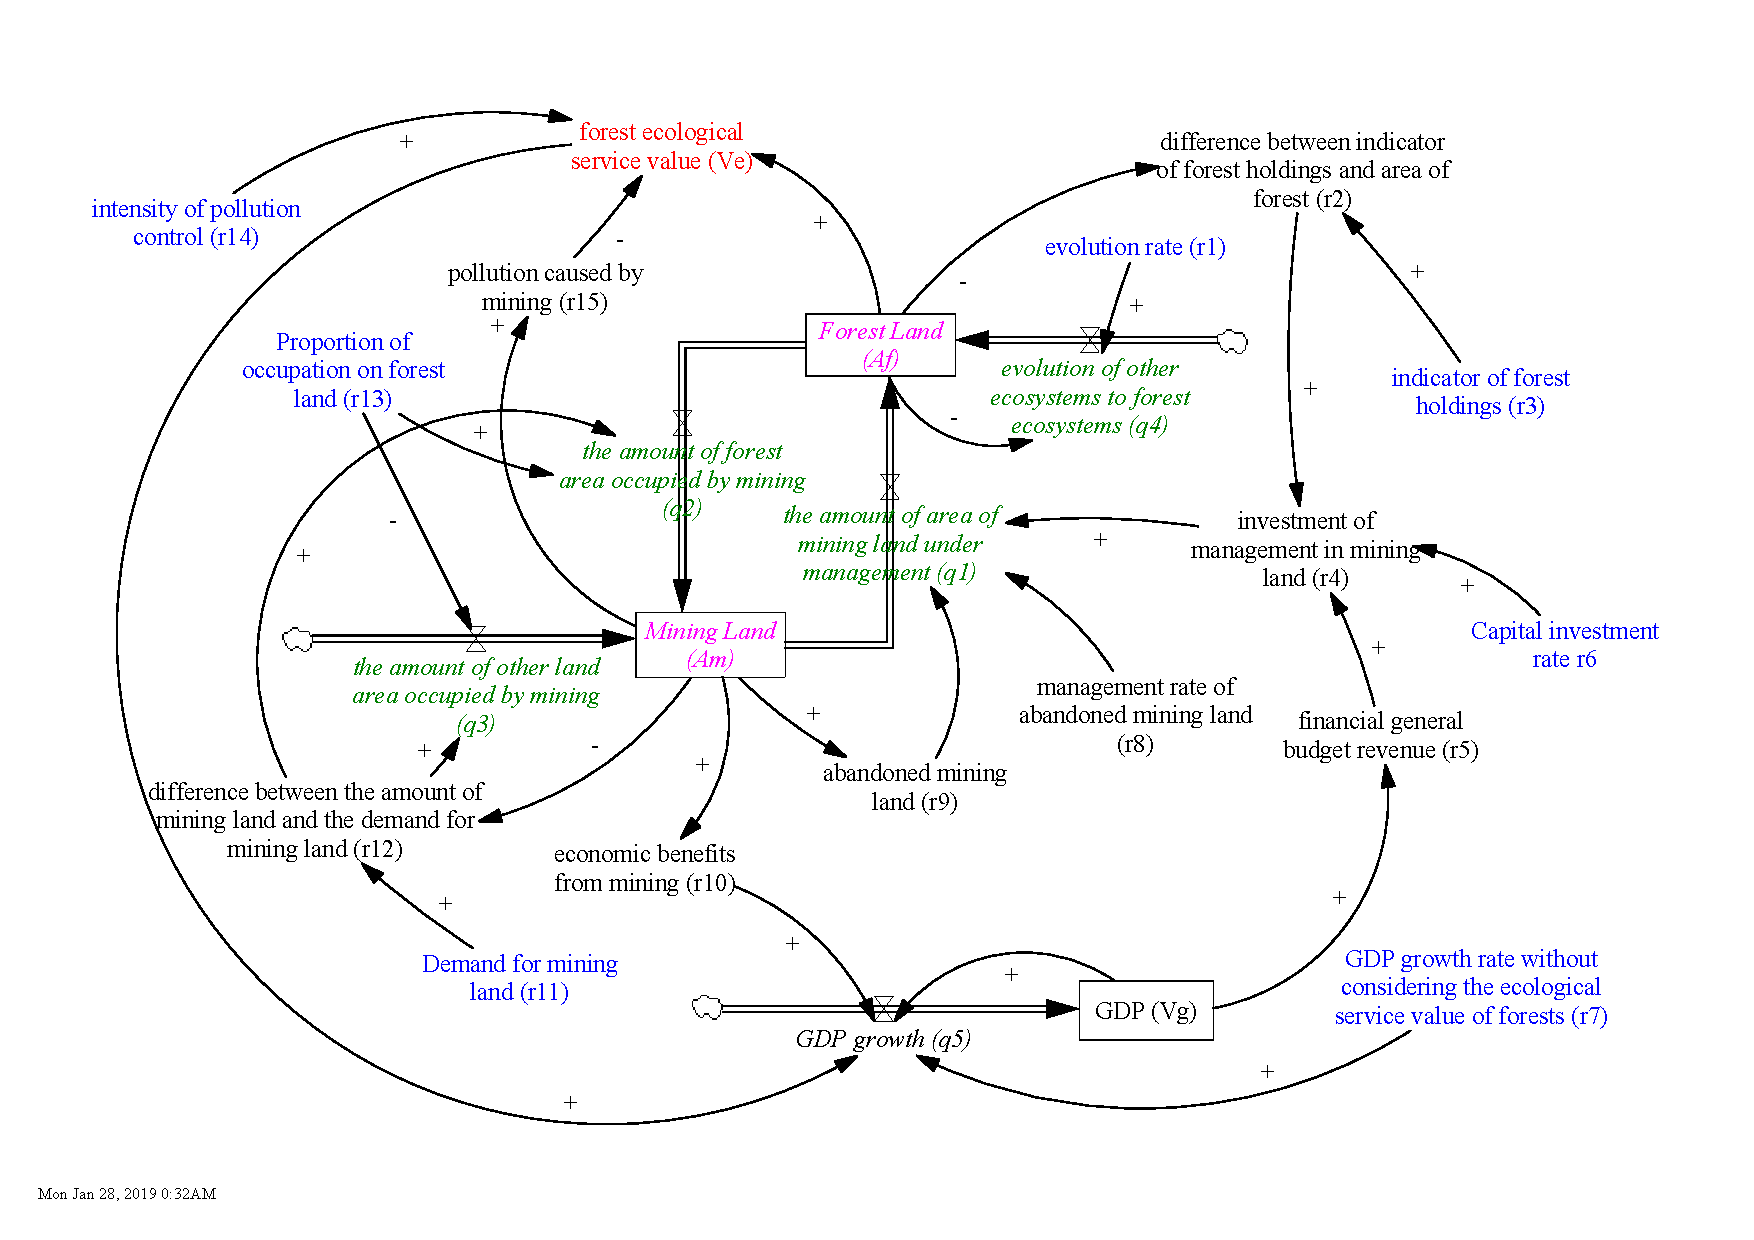
\includegraphics[width=\textwidth]{./pictures/dynamic.pdf}\\
  \caption{\small\heiti 森林生态系统土地面积变迁}\label{fig:dynamic}
\end{figure}

多图并列格式见图\,(\ref{fig:baifenbin})。

\begin{figure}[htbp]
\centering
\subfigure[\ce{CO2}]{
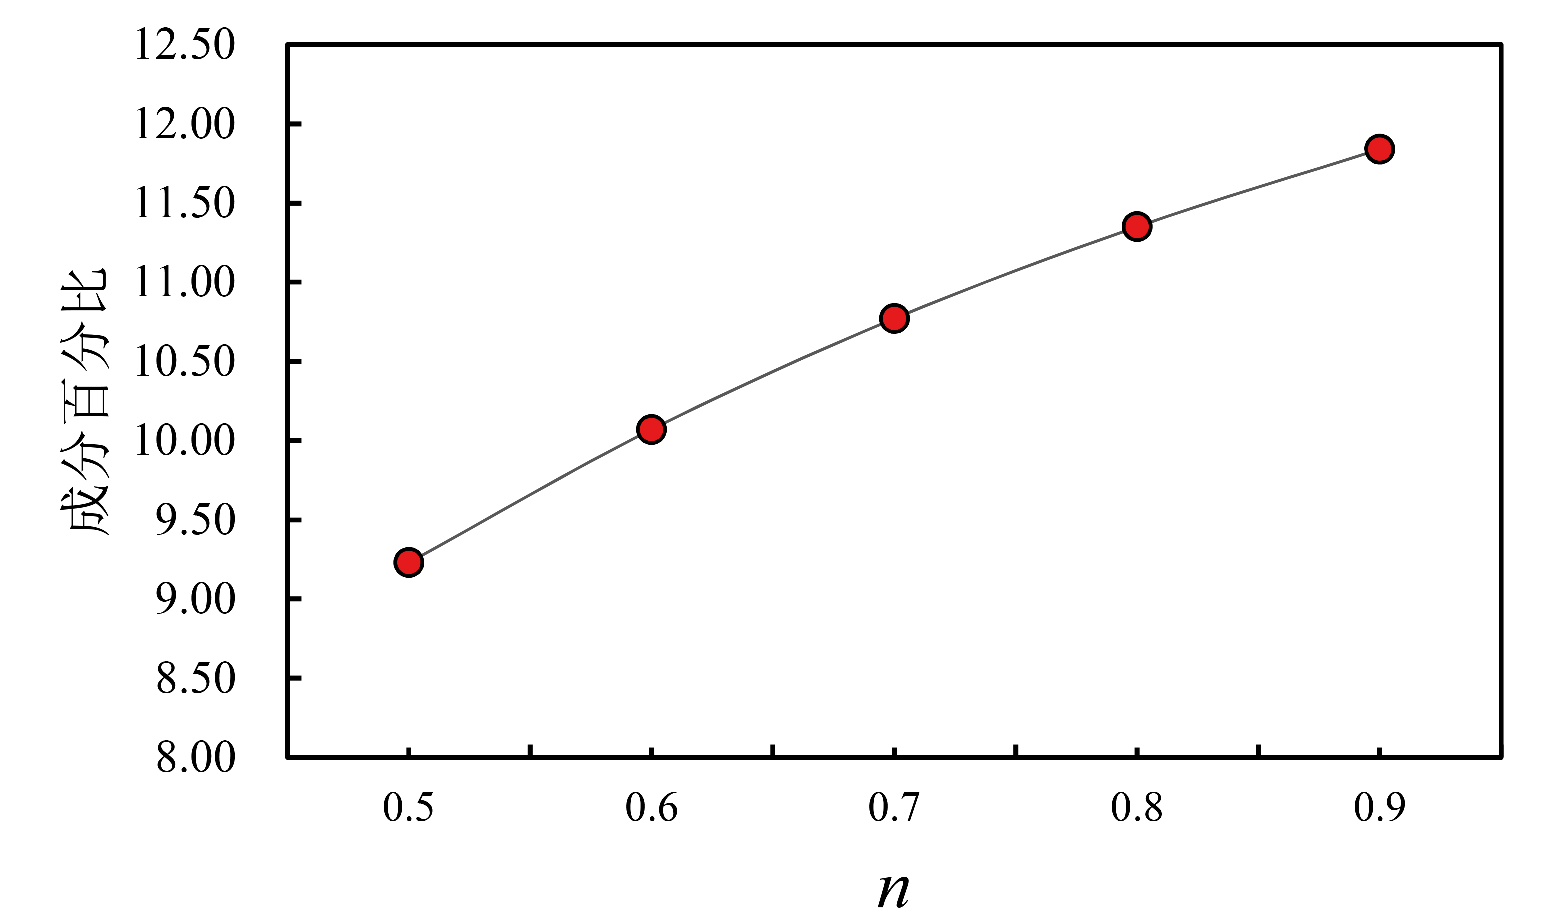
\includegraphics[width=0.46\textwidth]{./pictures/CO2.pdf}
}
\quad
\subfigure[\ce{CO}]{
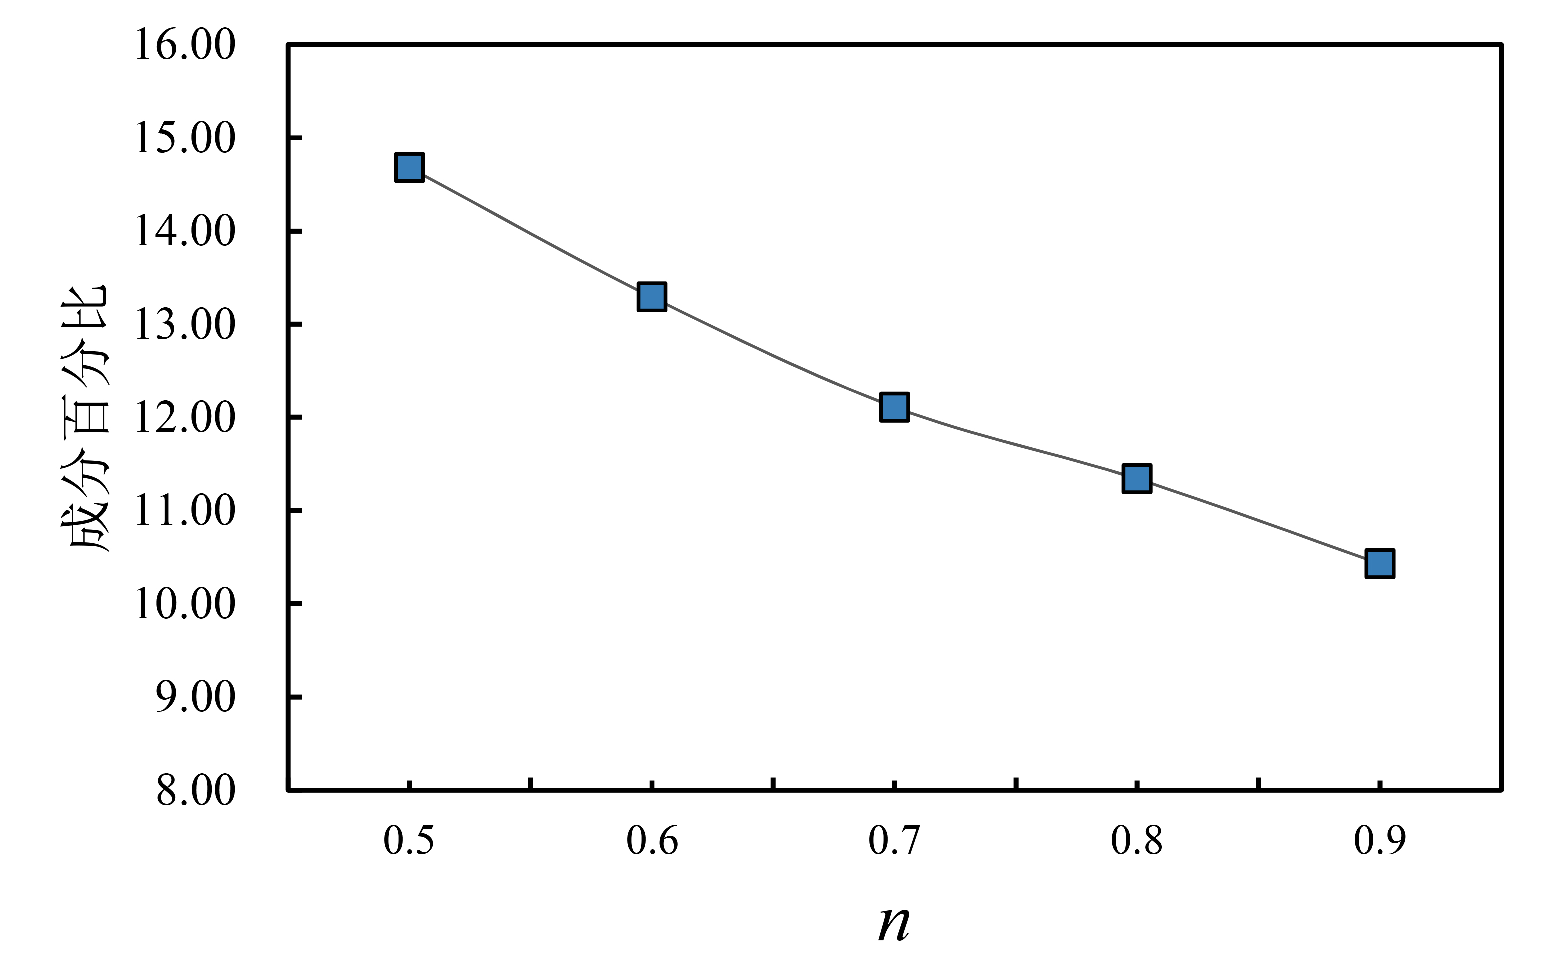
\includegraphics[width=0.46\textwidth]{./pictures/CO.pdf}
}
\quad
\subfigure[\ce{H2O}]{
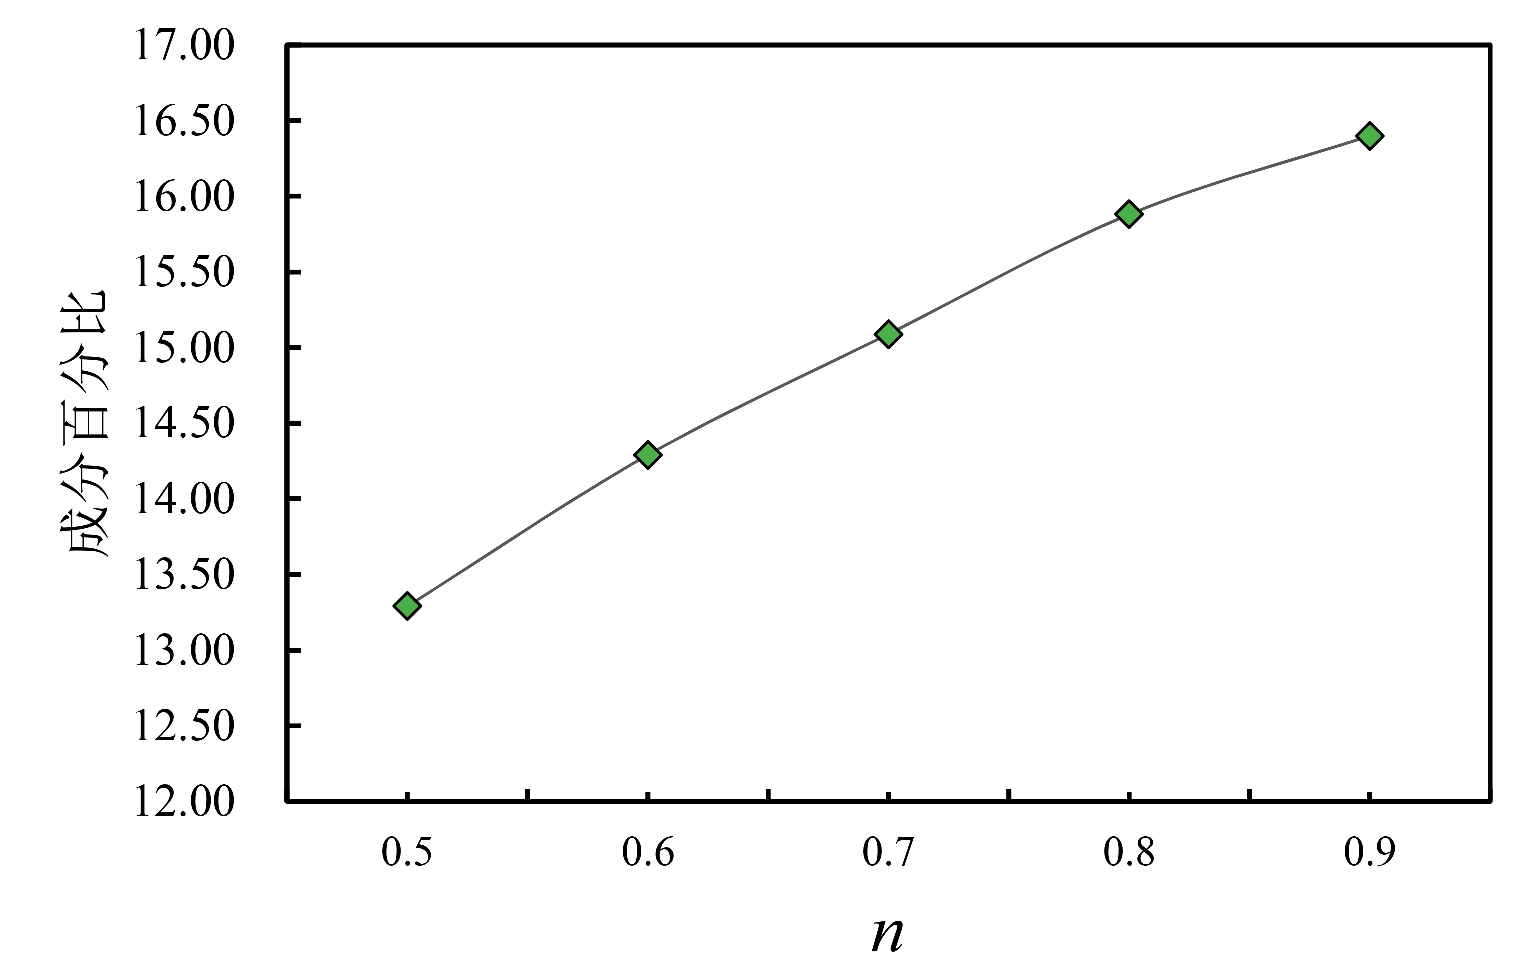
\includegraphics[width=0.46\textwidth]{./pictures/H2O.pdf}
}
\quad
\subfigure[\ce{H2}]{
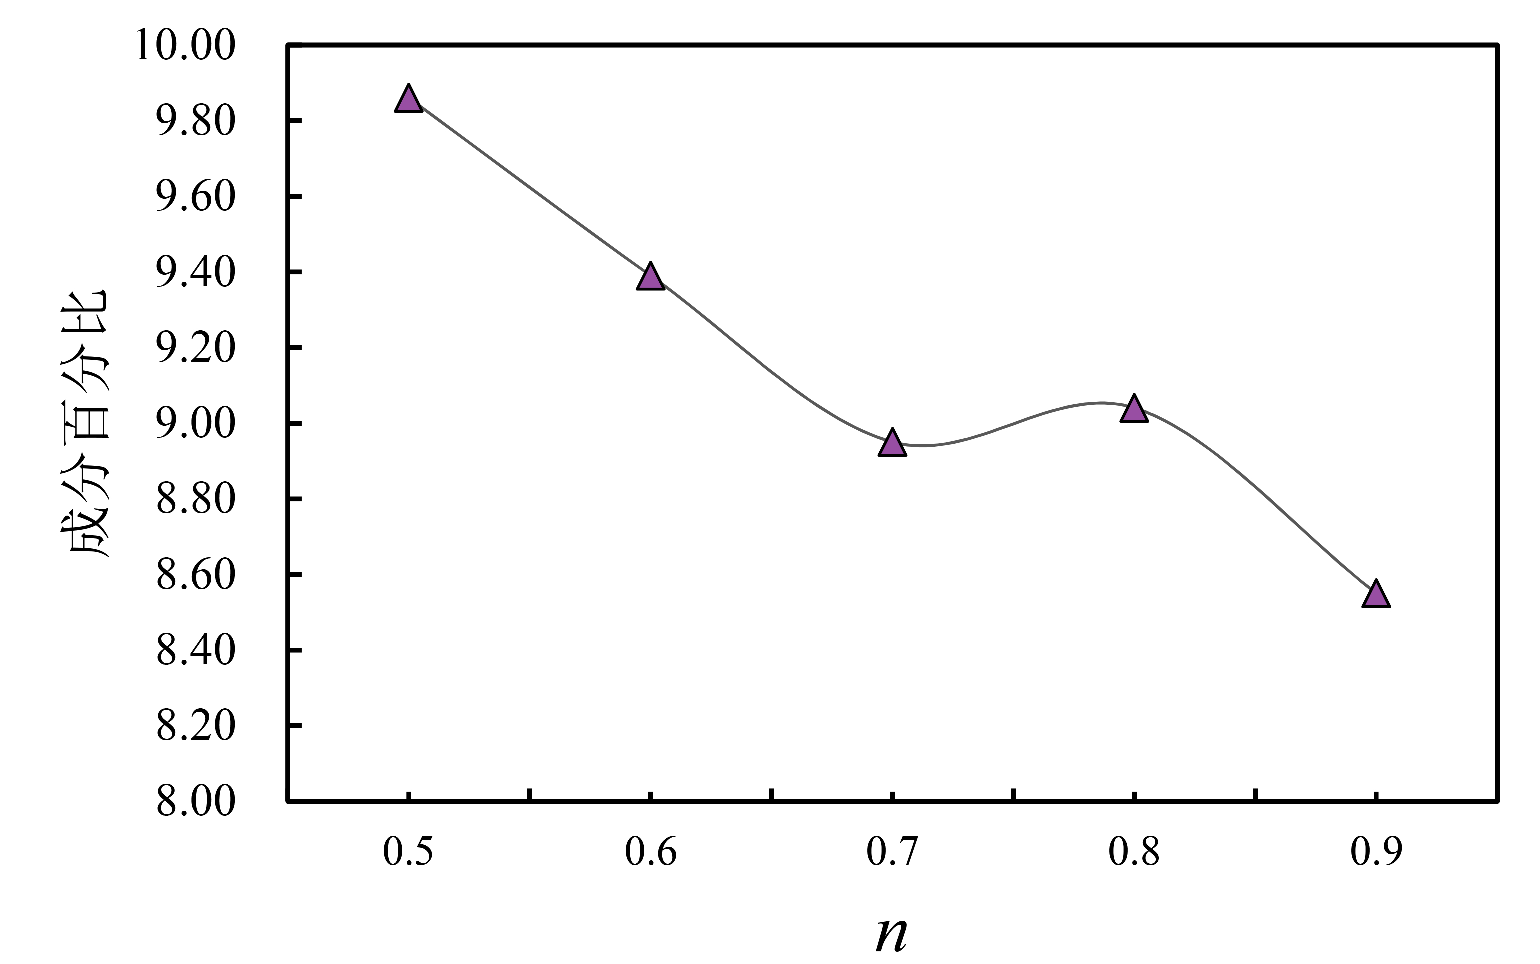
\includegraphics[width=0.46\textwidth]{./pictures/H2.pdf}
}
\quad
\subfigure[\ce{CH4}]{
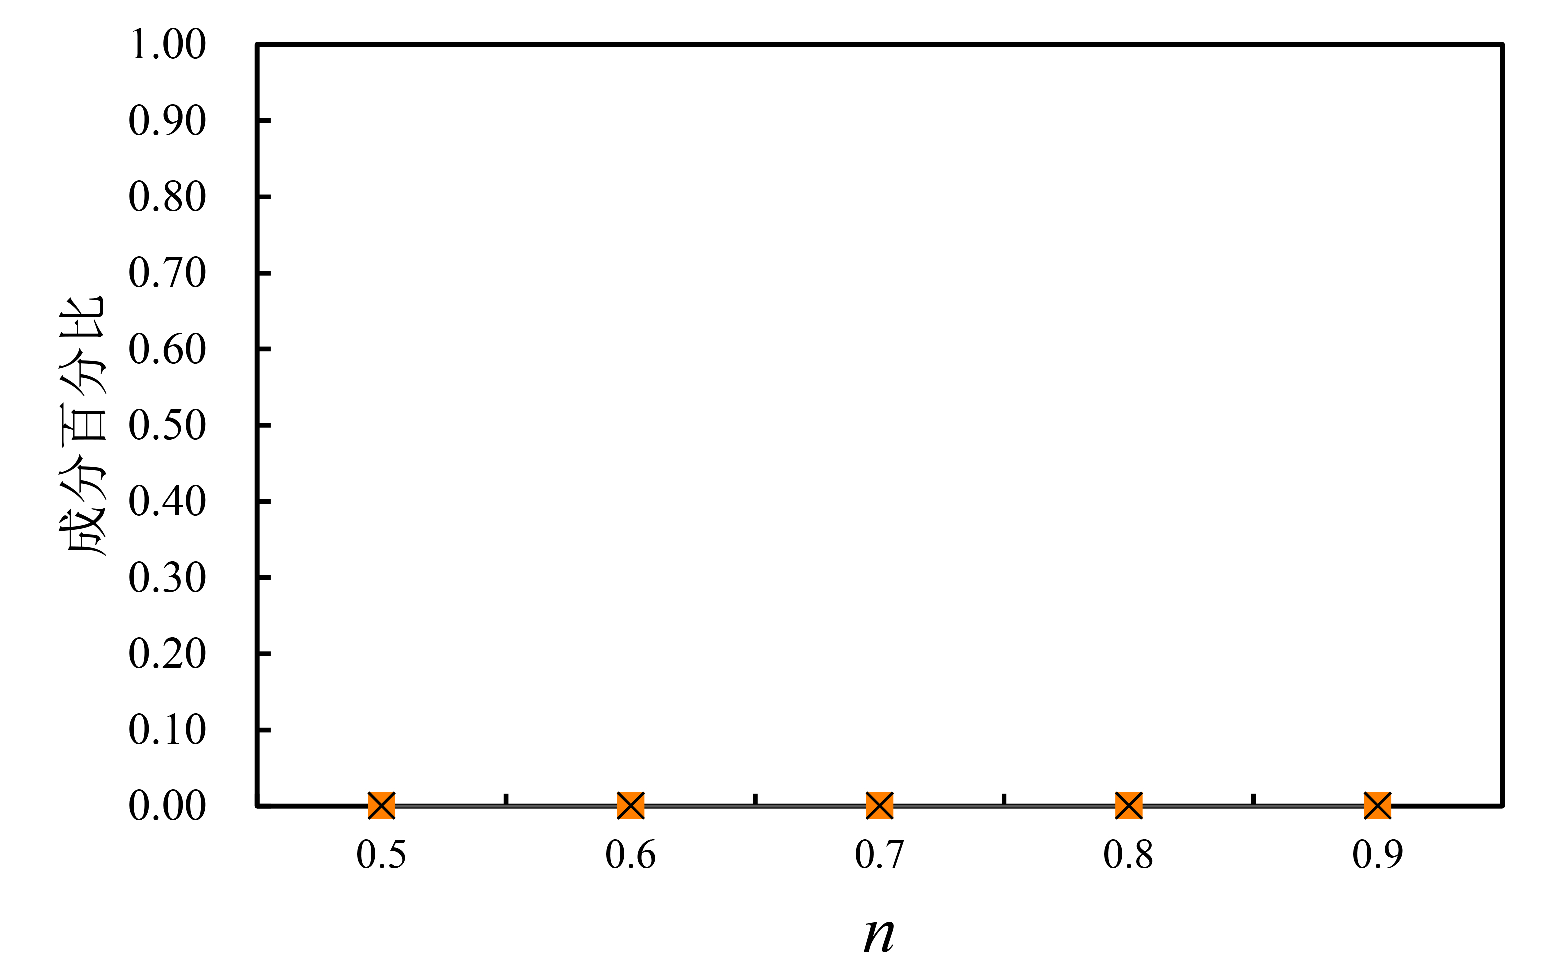
\includegraphics[width=0.46\textwidth]{./pictures/CH4.pdf}
}
\quad
\subfigure[\ce{N2}]{
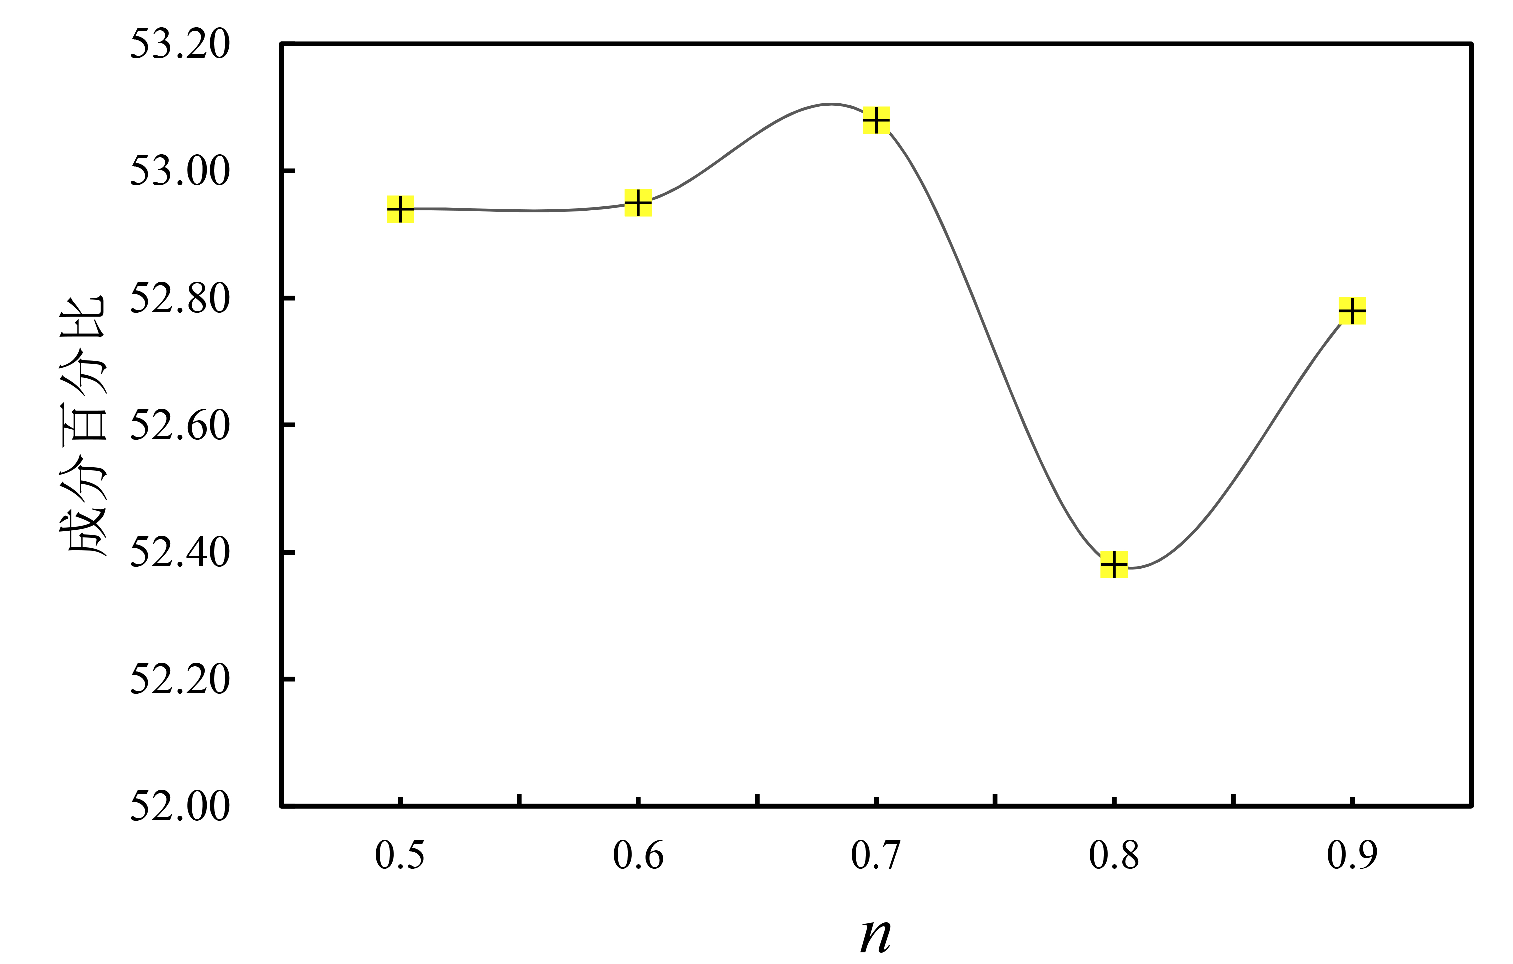
\includegraphics[width=0.46\textwidth]{./pictures/N2.pdf}
}
\caption{不完全燃烧产物成分百分比随$\,n\,$变化曲线图}\label{fig:baifenbin}
\end{figure}

\newpage\vspace*{-21.6pt}
\section{已知存在的问题}
本\LaTeX 模板中存在三个问题:

\begin{enumerate}[itemsep=0pt,parsep=0pt,label=\arabic*.]
  \item 目录中一级标题不是原Word文档中的“第1章\quad 概论”,而是“1\quad 概论”,但问题不大;
  \item 程序代码listings宏包与titletoc宏包疑似存在冲突(作者未找到具体起因),在排版程序代码时,可能报错:package inputenc error unicode char \verb"\u" 8 not set up use with latex,请谨慎使用listings宏包排版程序代码;
  \item 文献字体设置为楷体,而不是原Word文档中的楷体GB2312。
\end{enumerate}
